\renewcommand{\figwidth}{0.43\textwidth}
\begin{figure}[H]
	\centering
	\begin{subfigure}[b]{\figwidth}
		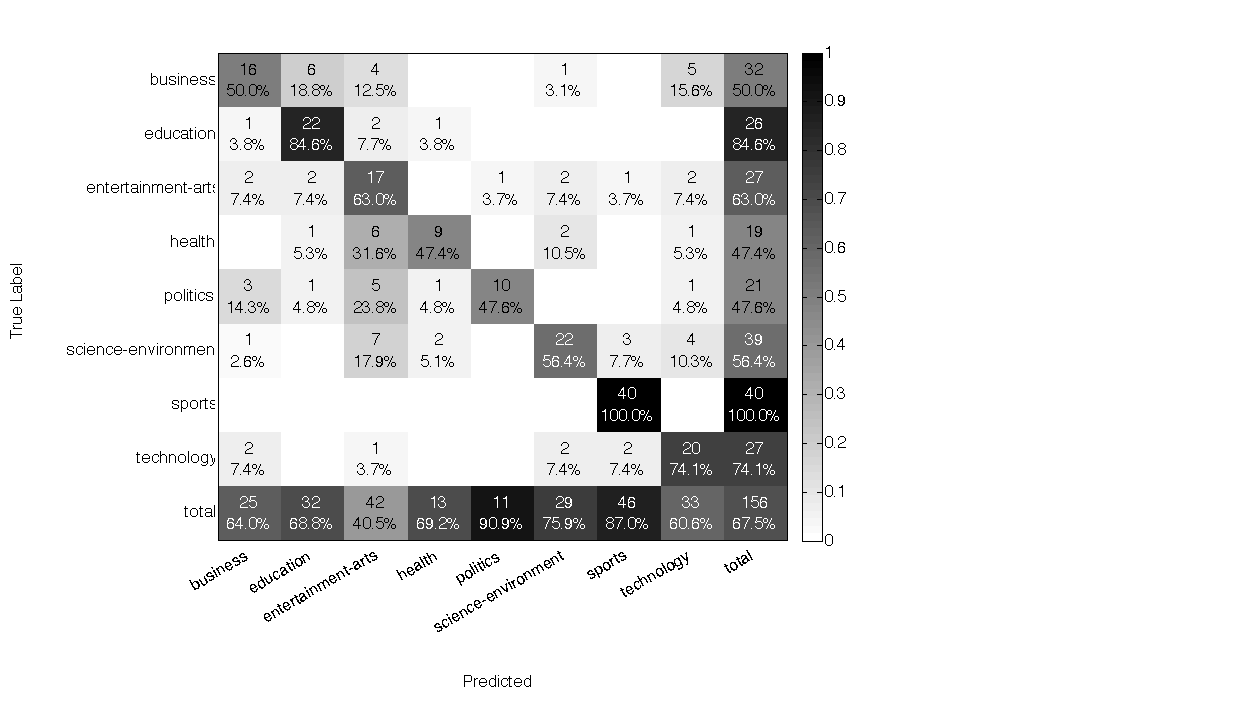
\includegraphics[width=\textwidth,trim=0 0 350 0, clip]{img/Bernou_percentile_5_count.png}
		\caption{Confusion matrix of Bernoulli.}
		\label{fig:confmat-be}
	\end{subfigure}
	~
	\begin{subfigure}[b]{\figwidth}
		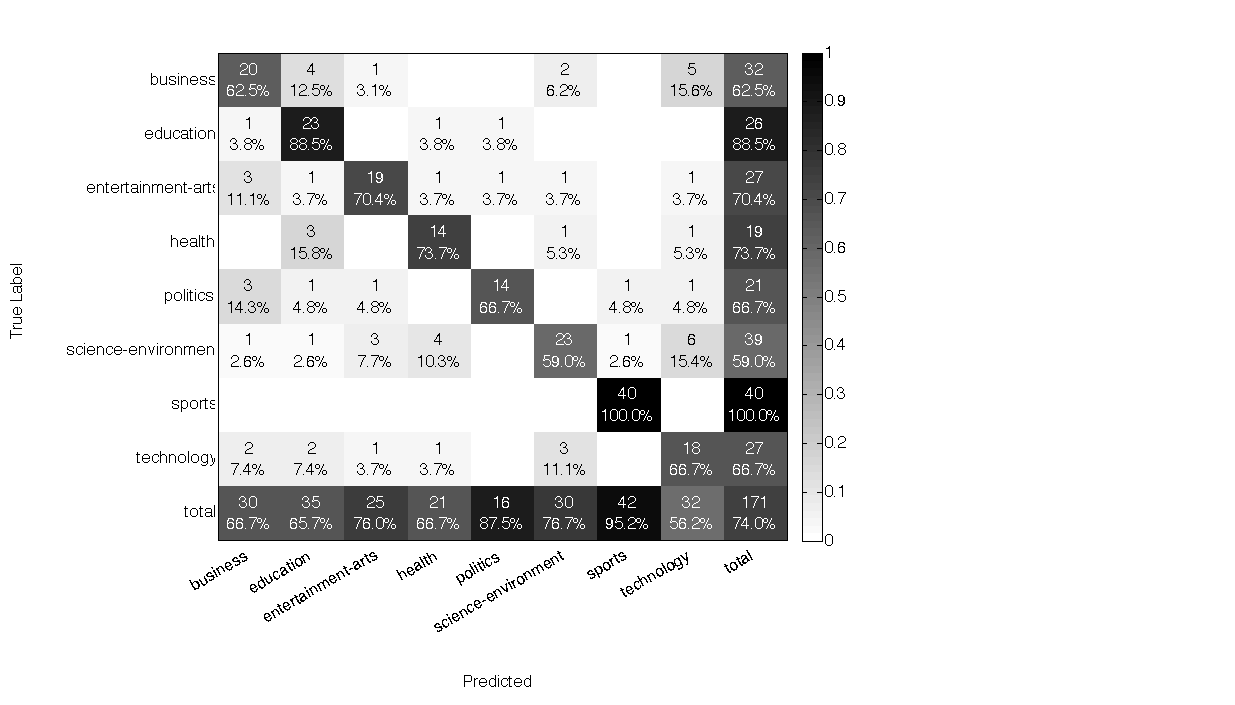
\includegraphics[width=\textwidth,trim=0 0 350 0, clip]{img/Multinomial_percentile_5_count.png}
		\caption{Confusion matrix of Multinomial.}
		\label{fig:confmat-mn}
	\end{subfigure}
	\\
	\begin{subfigure}[b]{\figwidth}
		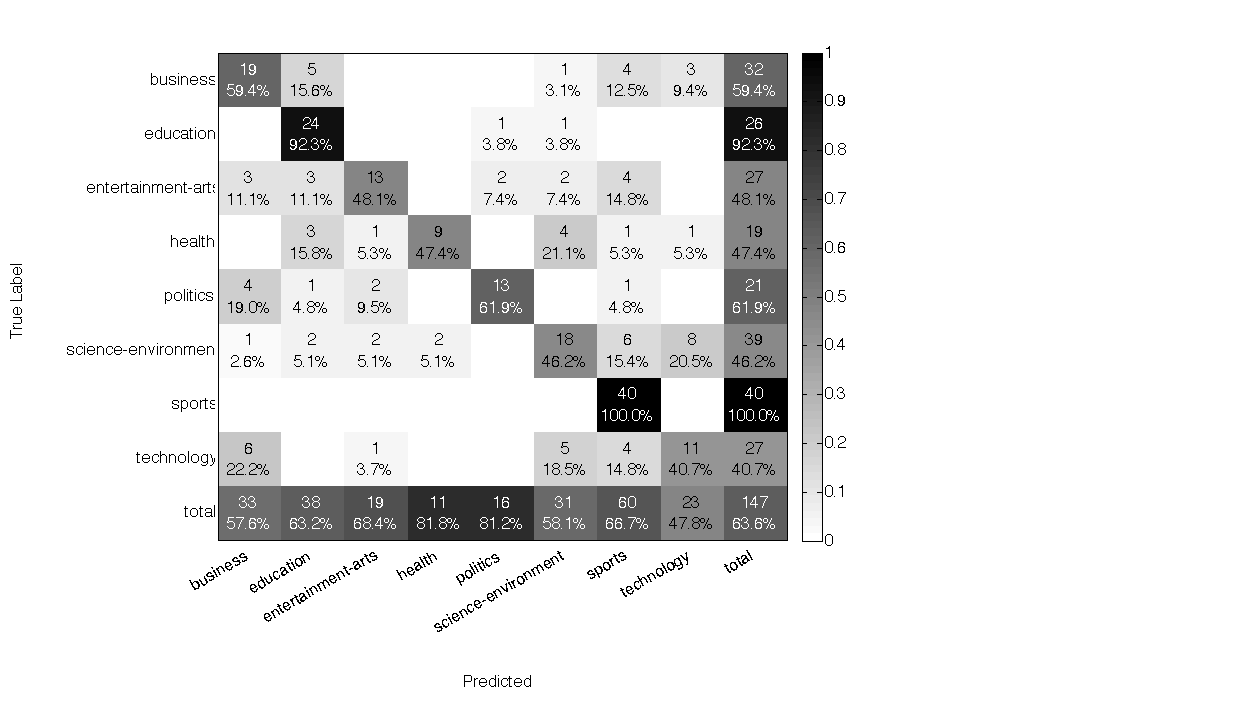
\includegraphics[width=\textwidth,trim=0 0 350 0, clip]{img/RandomForest_percentile_5_count.png}
		\caption{Confusion matrix of Random Forest.}
		\label{fig:confmat-rf}
	\end{subfigure}
	~
	\begin{subfigure}[b]{\figwidth}
		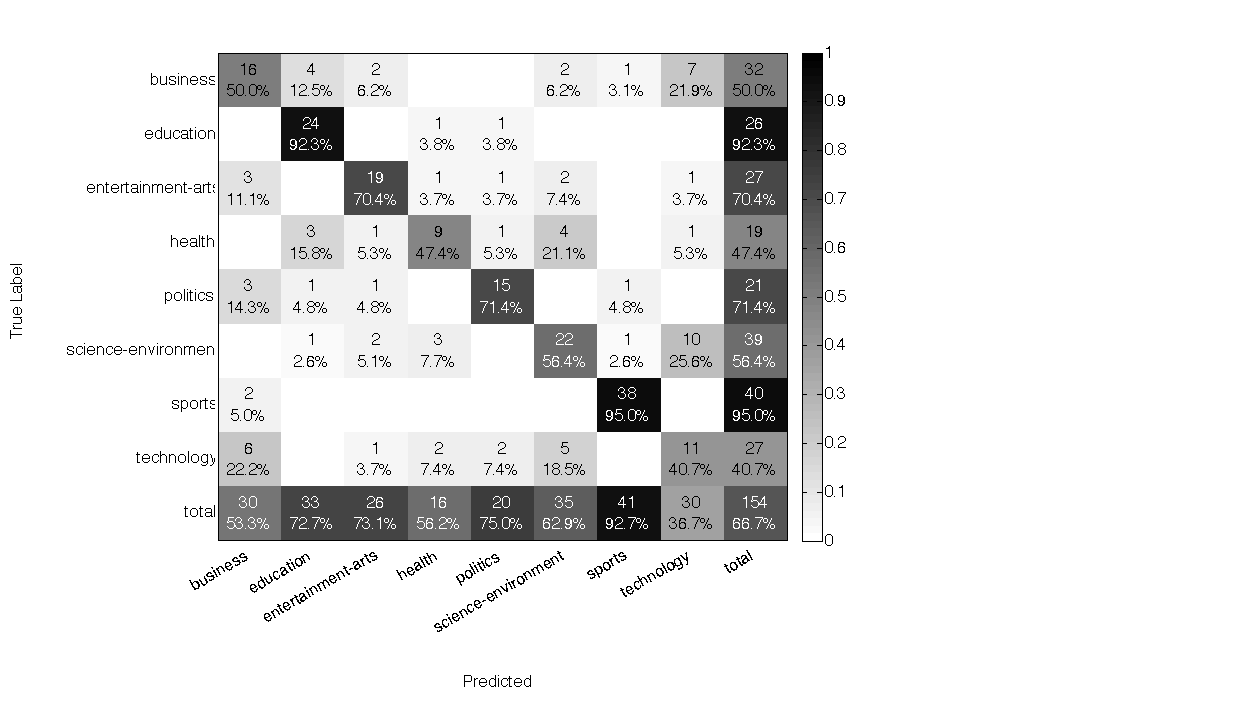
\includegraphics[width=\textwidth,trim=0 0 350 0, clip]{img/SVM_percentile_5_count.png}
		\caption{Confusion matrix of SVM.}
		\label{fig:confmat-svm}
	\end{subfigure}
	\\
	\begin{subfigure}[b]{\figwidth}
		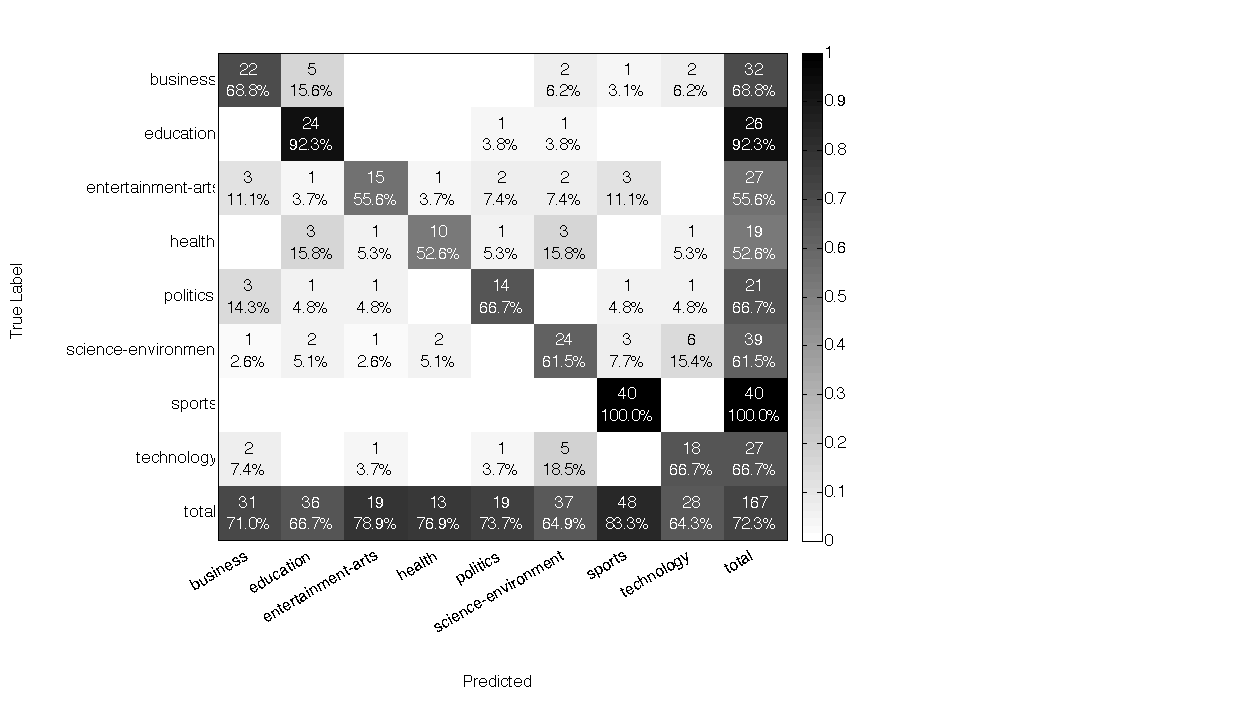
\includegraphics[width=\textwidth,trim=0 0 350 0, clip]{img/hybrid_percentile_5_count.png}
		\caption{Confusion matrix of Hybrid.}
		\label{fig:confmat-hybrid}
	\end{subfigure}
	\caption{Confusion matrices for the different classifiers. A total of 231 articles were tested. A vocabulary size of 511 words and the data type \emph{"Mapped value form 0 to 1"} were used.}
	\label{fig:confmat}
\end{figure}
